\chapter{Magnetic microscopy data application for Vredefort sample}

The observed data were measured on a regular grid of $121 \times 99$ (a total number of $N = 11979$ observations) over an area extending $\sim 36 \, mm$ and $\sim 30 \, mm$ along the x- and y-axis, respectively (Figure \ref*{fig:data_fitting}a). The sensor-to-sample distance was $138$ microns above the sample surface. We use a layer composed by a grid of $121 \times 99$ dipoles (a total of $M=11979$ equivalent sources) positioned at a constant depth of $z=750$ microns. The magnetization direction for all dipoles composing the equivalent layer is equal to $90^\circ$ and $0^\circ$ for inclination and declination, respectively. That is, its the same direction of the imparted field. 

By solving the equation \ref*{eq:ls_estimator}, using a regularizing parameter $\mu = 10^{-19}$, we estimate a magnetic-moment distribution over the layer (not shown). Figure \ref*{fig:data_fitting}b is the predicted data produced by equivalent layer. Figure \ref*{fig:data_fitting}c shows the residuals map that is the difference between observed data (Figure \ref*{fig:data_fitting}a) and the pŕedicted data (Figure \ref*{fig:data_fitting}b). The histogram of residuals appears with mean $0 \, mT$ and standard deviation $0,002 \, mT$. It means that the estimate magnetic-moment distribution produces an acceptable data fitting. Figure \ref*{fig:total_field_components}a, \ref*{fig:total_field_components}b and \ref*{fig:total_field_components}c show the predicted z-, x- and y-components of the magnetic field, respectively. We calculate the amplitude of total field using the estimated three components (Figure \ref*{fig:total_field_components}d). As we can notice from the amplitude of total field, there is a concentration of magnetic carriers on the upper bound of the Vredefort sample.      


%%%%%%%%%% Figures %%%%%%%%%%%%%
\begin{figure}[h!]
\centering
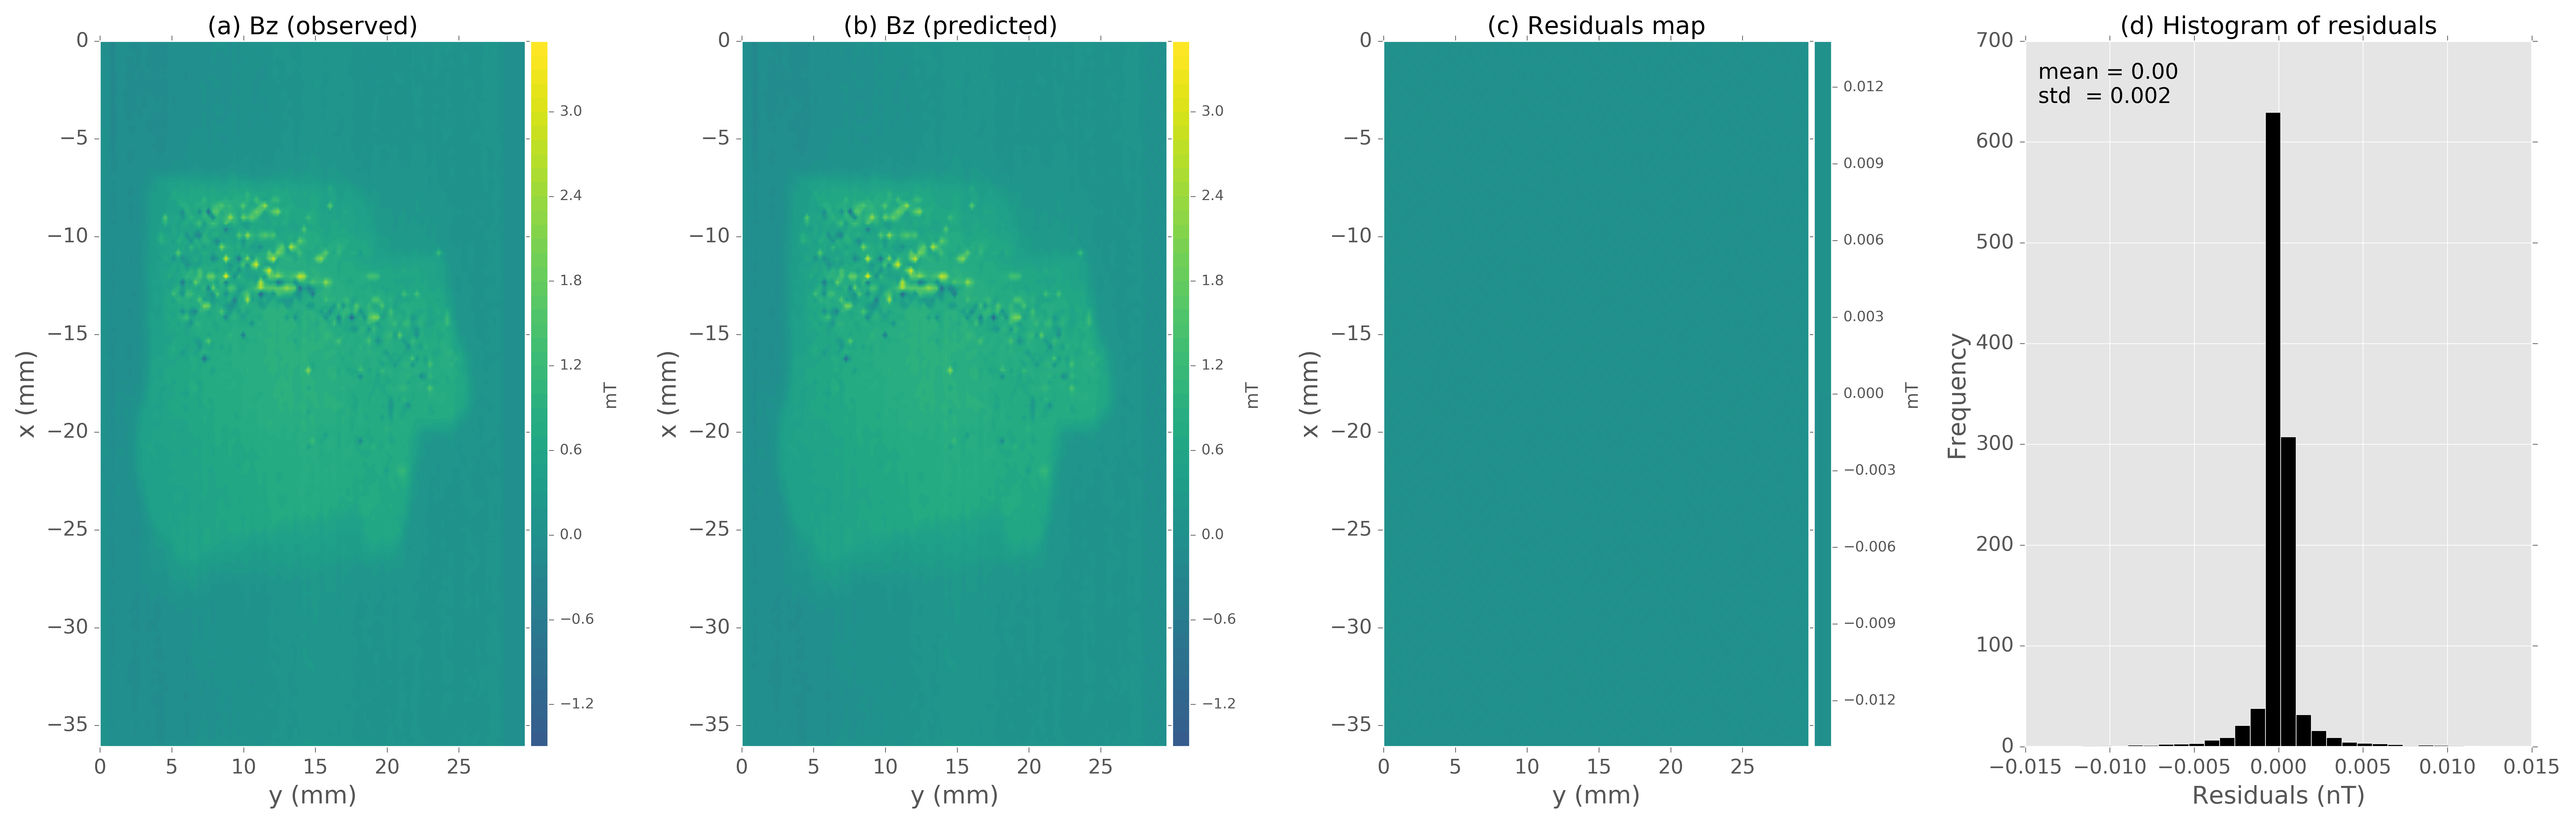
\includegraphics[width=0.8\textwidth]{vred/figs/results_data_fitting_eqlayer.png}
\caption{Application to microscopy data from Vredefort sample. (a) Observed z-component measured by magnetic microscope. (b) Estimated z-component produced by the model. (c) Difference between panels a and b. (d) Histogram of residuals. }
\label{fig:data_fitting}
\end{figure}

\begin{figure}[h!]
\centering
\includegraphics[width=0.6\textwidth]{vred/figs/field_components_eqlayer.png}
\caption{Application to microscopy data from Vredefort sample. (a) Map of z-component produced by the model. (b)  Map of estimated x-component. (c) Map of estimated y-component. (d) Total field calculated from the estimated magnetic-field components.}
\label{fig:total_field_components}
\end{figure}


 

